\section{Regressão Linear}

Nestes problemas, nós vamos explorar como Regressão Linear pode ser usada em tarefas de classificação.
Você usará o mesmo esquema de produção de pontos visto na parte acima do Perceptron, com $d = 2$,
$\mathcal{X} = [-1, 1] \times [-1, 1]$, e assim por diante.

newline \par
\textbf{Implementação:}



\begin{lstlisting}[language=Python, caption=Classificador por Regressão Linear, label=cod:reglin]
    # Classe para criar e treinar o classificador linear
    class Linear():
        def __init__(self):
            self.w = np.zeros(3)  # inicializa os pesos (incluindo o w_0)
        
        # Método para calcular a matriz X
        def calc_matriz_X(self, data):
            n_samples = len(data)
            X = np.hstack([np.ones((n_samples, 1)), data]) # adiciona coluna de 1s
            return X
        
        # Método para treinar o classificador linear
        def fit(self, data, labels):
            X = self.calc_matriz_X(data)
            y = labels
            X_T = np.transpose(X)
            X_pseudo_inv = np.dot(np.linalg.inv(np.dot(X_T, X)), X_T)
            self.w = np.dot(X_pseudo_inv, y)
            return self.w
        
        def classificar(self, data):
            X = self.calc_matriz_X(data)
            w_T = np.transpose(self.w)
            y_predicted = np.array([np.sign(np.dot(w_T, xn)) for xn in X])
            return y_predicted
\end{lstlisting}


\begin{enumerate}
    \item Considere $N = 100$. Use Regressão Linear para encontrar $g$ e calcule $E_{in}$, a fração de pontos dentro da amostra que foram classificados incorretamente (armazene os $g$'s pois eles serão usados no item seguinte). Repita o experimento 1000 vezes. Qual dos valores abaixo é mais próximo do $E_{in}$ médio?
    
    \begin{enumerate}
        \item 0
        \item 0.001
        \item[\textcolor{red}{(c)}]\textcolor{red}{0.01}\addtocounter{enumii}{1}
        \item 0.1
        \item 0.5
        % 
    \end{enumerate}
 
    \par

    \textbf{Justificativa:}

    Para responder a esse item foi implementada a seguinte função:

    \begin{lstlisting}[language=Python, caption=Cálculo do E\_in, label=cod:calc_E_in]
        def calc_E_in(num_points, verbose = True):
            lista_E_in = list()
            lista_target = list()
            lista_linear = list()
            for _ in range(1000):
                # Criar a função target
                target = Target()
                a, b = target.generate_random_line()
                # Criar o dataset
                dataset = Dataset(num_points)
                data, labels = dataset.generate_dataset(target)
                # Criar e treinar o classificador linear
                linear = Linear()
                w = linear.fit(data,labels)
                # Classificar os pontos
                y_predicted = linear.classificar(data)
                # Calcular E_in para essa execução
                lista_E_in.append(np.mean(labels != y_predicted))
                # Guardar para saida
                lista_target.append(target)
                lista_linear.append(linear)
            E_in = np.mean(lista_E_in)
            if verbose: print(f"E_in = {E_in:.4f}")
            return E_in, lista_target, lista_linear
    \end{lstlisting}

    Foram realizadas 1000 execuções e em cada uma foi gerada uma nova função target, um novo dataset e foi treinado um novo regressor linear. O $E_{in}$ em cada iteração foi calculado pelo número de erros dividido pela quantidade de pontos dentro da amostra. O valor final $E_{in} = 0.0420 = 4.20\%$ foi dado pela média dos $E_{in}$ em cada iteração. Como $0.0420$ está mais próximo de $0.01$ do que de $0.1$, o \textcolor{red}{item (c)} foi o escolhido.

    \item Agora, gere 1000 pontos novos e use eles para estimar o $Eout$ dos $g$'s que você encontrou no item anterior. Novamente, realize 1000 execuções. Qual dos valores abaixo é mais próximo do $E_{out}$ médio?
    
    \begin{enumerate}
        \item 0
        \item 0.001
        \item[\textcolor{red}{(c)}]\textcolor{red}{0.01}\addtocounter{enumii}{1}
        \item 0.1
        \item 0.5
    \end{enumerate}

    \par

    \textbf{Justificativa:}

    Para responder a esse item foi implementada a seguinte função:

    \begin{lstlisting}[language=Python, caption=Cálculo do E\_out, label=cod:calc_E_out]
        def calc_E_out(num_points, lista_target, lista_linear, verbose = True):
            lista_E_out = list()
            for target, linear in zip(lista_target, lista_linear):
                # Criar o dataset com a mesma função target do E_in
                dataset = Dataset(num_points)
                data, labels = dataset.generate_dataset(target)
                # Classificar os pontos com a mesma hipótese do E_in
                y_predicted = linear.classificar(data)
                # Calcular E_out para essa execução
                lista_E_out.append(np.mean(labels != y_predicted))
            E_out = np.mean(lista_E_out)
            if verbose: print(f"E_out = {E_out:.4f}")
            return E_out
    
    \end{lstlisting}

    Como o enunciado pede explicitamente que sejam utilizados os mesmos $g$'s do item anterior, a função no código \ref{cod:calc_E_out} recebe como entrada os targets e as hipóteses calculadas no item anterior (e que por isso foram colocadas como saída na função apresentada no código \ref{cod:calc_E_in}). Foram realizadas 1000 execuções e em cada uma foi gerado um novo dataset com 1000 pontos utilizando um dos targets gerados no item anterior e classificados pela hipótese treinada no item anterior para o mesmo target. O $E_{out}$ em cada iteração foi calculado pelo número de erros dividido pela quantidade de pontos no dataset. O valor final $E_{out} = 0.0489 = 4.89\%$ foi dado pela média dos $E_{out}$ em cada iteração. Como $0.0489$ está mais próximo de $0.01$ do que de $0.1$, o \textcolor{red}{item (c)} foi o escolhido.

    \item Agora, considere $N = 10$. Depois de encontrar os pesos usando Regressão Linear, use-os como um vetor de pesos iniciais para o Algoritmo de Aprendizagem Perceptron (PLA). Execute o PLA até que ele convirja num vetor final de pesos que separa perfeitamente os pontos dentro-de-amostra. Dentre as opções abaixo, qual é mais próxima do número médio de iterações (sobre 1000 execuções) que o PLA demora para convergir?
    
    \begin{enumerate}
        \item [\textcolor{red}{(a)}]\textcolor{red}{1}\addtocounter{enumii}{1}
        \item 15
        \item 300
        \item 5000
        \item 10000
    \end{enumerate}

    \par

    \textbf{Justificativa:}

    Para responder a esse item foi implementada a seguinte função:

    \begin{lstlisting}[language=Python, caption=Cálculo do número de iterações do PLA, label=cod:calc_PLA_iter]
        def calc_PLA_iter(num_points):
            lista_iter = list()
            for _ in range(1000):
                # Criar a função target
                target = Target()
                target.generate_random_line()
                # Criar o dataset
                dataset = Dataset(num_points)
                data, labels = dataset.generate_dataset(target)
                # Criar e treinar o classificador linear
                linear = Linear()
                w = linear.fit(data,labels)
                # Criar e treinar o perceptron
                perceptron = Perceptron2D(weights=w)
                iter, _ = perceptron.pla(data,labels)
                lista_iter.append(iter)
            print(f"{np.mean(lista_iter)} iterações com desvio padrão {np.std(lista_iter):.4f} (min:{np.min(lista_iter)}, máx:{np.max(lista_iter)})")
    \end{lstlisting}

    Foram realizadas 1000 execuções e em cada uma foi gerada uma nova função target e um novo dataset com 10 pontos. Em cada iteração é treinado um Classificador Linear e seus pesos são utilizados como pesos iniciais para treinar um Perceptron 2D. O número de iterações internas realizadas no método $perceptron.pla(data,labels)$, que treina o Perceptron utilizando o PLA, é armazenado em uma lista e no final das execuções é calculada a média e o desvio padrão desses valores. O resultado após 1000 execuções do experimento foi uma média de $3.1460(\approx 3)$ iterações, com desvio padrão de $7.8247(\approx 8)$ iterações, mínimo de 1 iteração e máximo de 104 iterações. Ainda é possível observar uma grande variação do número de iterações entre cada execução, porém a média é menor do que a calculada no item 1 do problema 1 $(\approx 5)$. É possível constatar então que o PLA converge mais rápido quando seus pesos são inicializados por uma Regressão Linear. Como 3 está mais próximo de 1 do que de 15, o \textcolor{red}{\textbf{item a}} foi selecionado. 
    
    \item Vamos agora avaliar o desempenho da versão pocket do PLA em um conjunto de dados que não é linearmente separável. Para criar este conjunto, gere uma base de treinamento com $N_1$ pontos como foi feito até agora, mas selecione aleatoriamente 10\% dos pontos e inverta seus rótulos. Em seguida, implemente a versão pocket do PLA, treine-a neste conjunto não-linearmente separável, e avalie seu $E_{out}$ numa nova base de $N_2$ pontos na qual você não aplicará nenhuma inversão de rótulos. Repita para 1000 execuções, e mostre o $E_{in}$ e $E_{out}$ médios para as seguintes configurações (não esqueça dos gráficos scatterplot, como anteriormente):
    
    \par

    \textbf{Implementação:}
    
    Para responder os subitens abaixo, foi adicionado à classe Perceptron2D (código \ref{cod:perceptron}), utilizada no problema 1, um método para fazer o treinamento utilizando o algoritmo Pocket (código \ref{cod:pocket}) e foi implementada também uma função para calcular o $E_{in}$ e $E_{out}$ médio (código \ref{cod:calc_pocket_E}) em 1000 execuções de treinamento do Perceptron utilizando o algoritmo Pocket. A função permite escolher se irá ou não utilizar os pesos de um classificador linear como pesos iniciais do perceptron e também plota o dataset com a Função Target e a Hipótese para a última execução.

    \begin{lstlisting}[language=Python, caption=Algoritmo Pocket, label=cod:pocket]
        # Método para treinar o perceptron usando o algoritmo Pocket
        def pocket(self, data, labels, max_iter = 1000): 
            n_samples = len(data)
            X_bias = np.hstack([np.ones((n_samples, 1)), data]) # adiciona uma coluna de 1s para o X_0 (coordenada artificial)
            iterations = 0
            E_in = 1
            w = self.w
            while E_in > 0 and iterations < max_iter:
                E_in_atual = 0
                w_atual = w
                errors = 0
                for i in range(n_samples):
                    if labels[i] * np.dot(self.w, X_bias[i]) <= 0:
                        w_atual += labels[i] * X_bias[i] # atualiza os pesos
                        errors += 1
                iterations += 1
                E_in_atual = errors/n_samples
                if E_in_atual < E_in: # atualiza os pesos e o E_in apenas se o E_in for menor que o anterior
                    E_in = E_in_atual
                    w = w_atual
            self.w = w
            return iterations, self.w, E_in
        setattr(Perceptron2D, "pocket", pocket)
    \end{lstlisting}

    \begin{lstlisting}[language=Python, caption=Cálculo do E\_in e do E\_out, label=cod:calc_pocket_E]
        def calc_pocket_E(N1, N2, i, LinReg = False):
            lista_E_in = list()
            lista_E_out = list()
            for _ in range(1000):
                # Criar a função target
                target = Target()
                a, b = target.generate_random_line()
                # Criar o dataset de treinamento
                dataset_train = Dataset(N1)
                x_train, y_train = dataset_train.generate_dataset(target)
                selected_indices = np.random.choice(len(y_train), int(len(y_train) * 0.1), replace=False) # seleciona 10%
                y_train[selected_indices] *= -1 # inverte o valor de 10%
                if LinReg: # pesos inicializados com regressão linear
                    # Criar e treinar o classificador linear
                    linear = Linear()
                    w = linear.fit(x_train,y_train)
                    # Criar e treinar o perceptron com pocket
                    perceptron = Perceptron2D(weights=w)
                    _, _, E_in = perceptron.pocket(x_train,y_train, max_iter = i)
                    lista_E_in.append(E_in)
                else: # pesos inicializados com 0
                    # Criar e treinar o perceptron com pocket
                    perceptron = Perceptron2D()
                    _, _, E_in = perceptron.pocket(x_train,y_train, max_iter = i)
                    lista_E_in.append(E_in)
                # Criar o dataset de teste
                dataset_test = Dataset(N2)
                x_test, y_test = dataset_test.generate_dataset(target)
                # Classificar os pontos com a mesma hipotese do E_in
                y_predicted = perceptron.classificar(x_test)
                # Calcular E_out para essa execução
                E_out = np.mean(y_test != y_predicted)
                lista_E_out.append(E_out)
            # Printar E_in e E_out médios
            print(f"E_in = {np.mean(E_in):.4f}")
            print(f"E_out = {np.mean(E_out):.4f}")
            # Plotar o dataset, a função target e a hipótese g da última execução
            scatterplot(x_train, y_train, target, perceptron)
    \end{lstlisting}

    
    \begin{enumerate}
        \item Inicializando os pesos com 0; $i = 10$; $N_1 = 100$; $N_2 = 1000$.
        
        \textbf{Resposta:} $E_{in} = 0.2200$ e $E_{out} = 0.2540$.

        \begin{figure}[H]
            \caption{Base de dados de treinamento inicializando os pesos com 0 e $i = 10$}
               \centering
               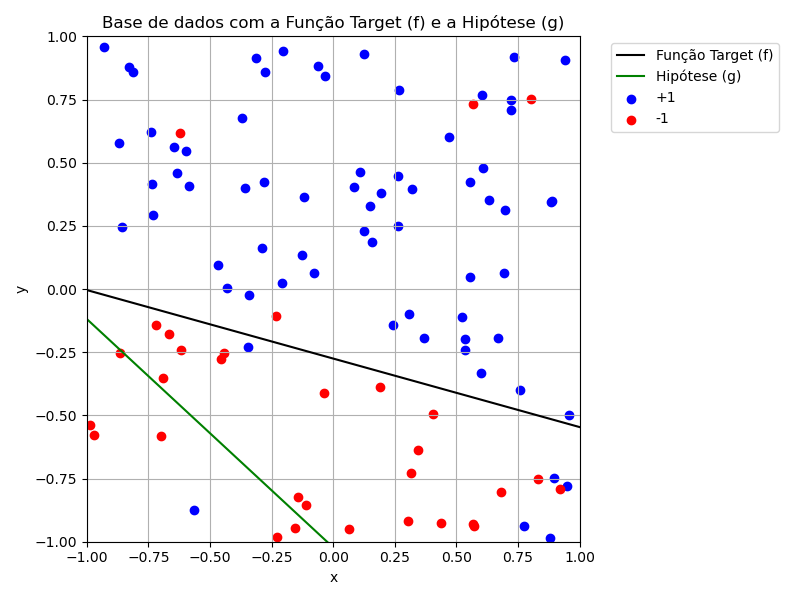
\includegraphics[width=12cm]{pocket_i10_w0.png}
        \end{figure}

        \item Inicializando os pesos com 0; $i = 50$; $N_1 = 100$; $N_2 = 1000$.
        
        \textbf{Resposta:} $E_{in} = 0.2400$ e $E_{out} = 0.0350$.

        \begin{figure}[H]
            \caption{Base de dados de treinamento inicializando os pesos com 0 e $i = 50$}
               \centering
               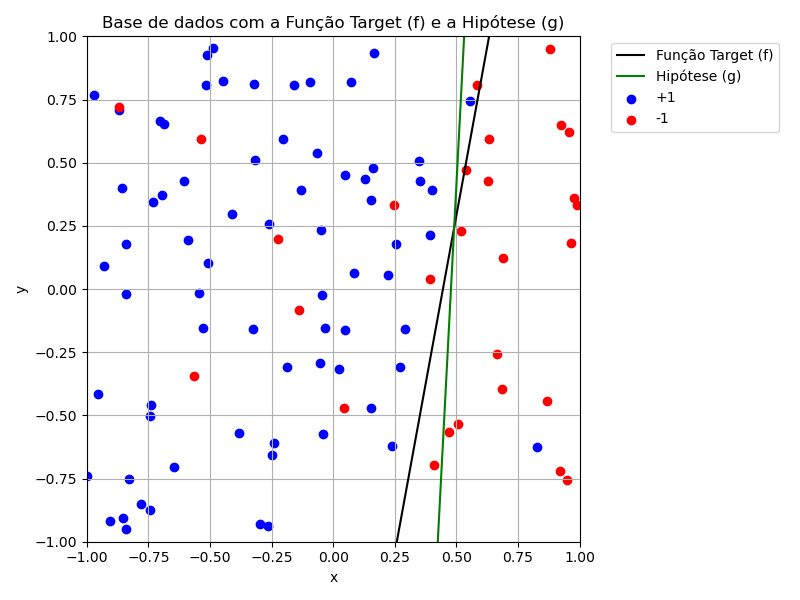
\includegraphics[width=12cm]{pocket_i50_w0.png}
        \end{figure}

        \item Inicializando os pesos com Regressão Linear; $i = 10$; $N_1 = 100$; $N_2 = 1000$.
        
        \textbf{Resposta:} $E_{in} = 0.2200$ e $E_{out} = 0.01400$.

        \begin{figure}[H]
            \caption{Base de dados de treinamento inicializando os pesos com Regressão Linear e $i = 10$}
               \centering
               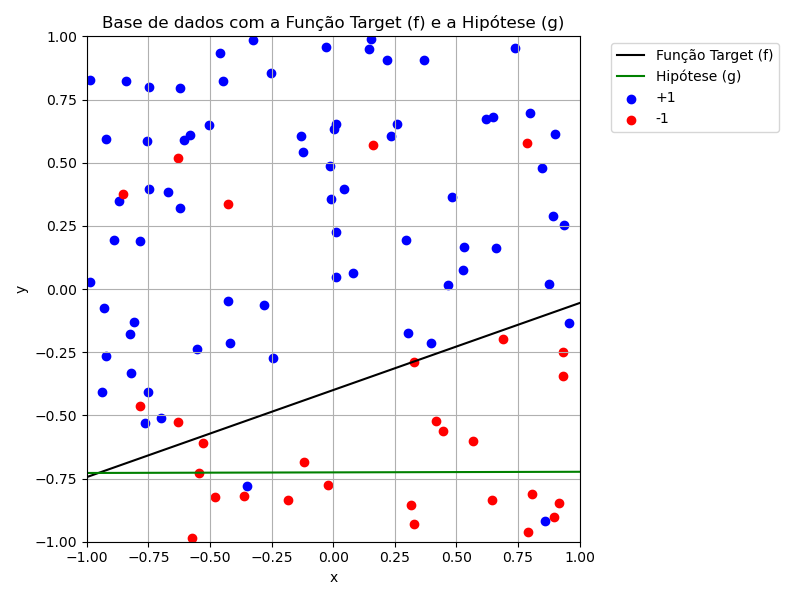
\includegraphics[width=12cm]{pocket_i10_reglin.png}
        \end{figure}

        \item Inicializando os pesos com Regressão Linear; $i = 50$; $N_1 = 100$; $N_2 = 1000$.

        \textbf{Resposta:} $E_{in} = 0.1800$ e $E_{out} = 0.0880$.

        \begin{figure}[H]
            \caption{Base de dados de treinamento inicializando os pesos com Regressão Linear e $i = 50$}
               \centering
               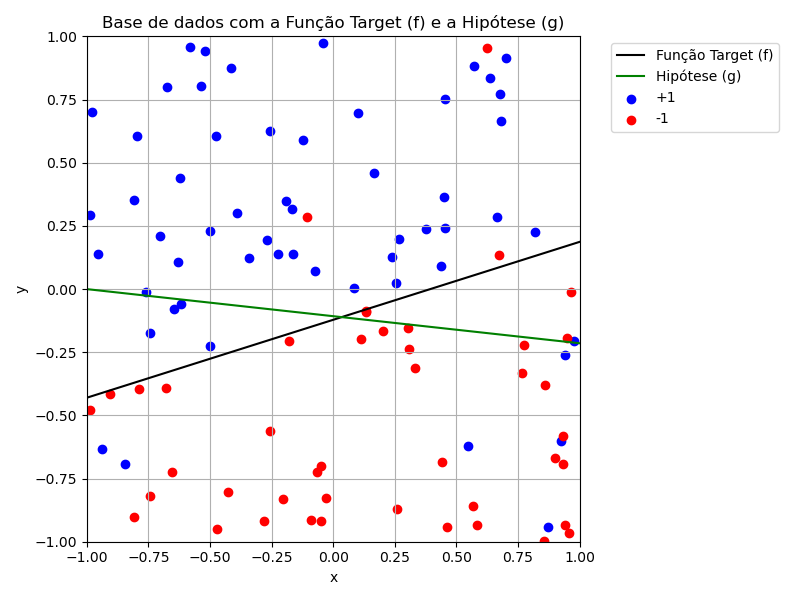
\includegraphics[width=12cm]{pocket_i50_reglin.png}
        \end{figure}

        \textbf{Comentários sobre os 4 subitens:} Para todos os subitens o $E_{out}$ foi menor do que o $E_{in}$, o que normalmente não ocorre, porém neste experimento se Justifica pelo fato do dataset de treinamento (dentro da amostra) ter sofrido inversões de labels e o dataset de teste (fora da amostra) não. 

    \end{enumerate}

    
\end{enumerate}